\section{Method}


\begin{figure}[t]
    \centering
    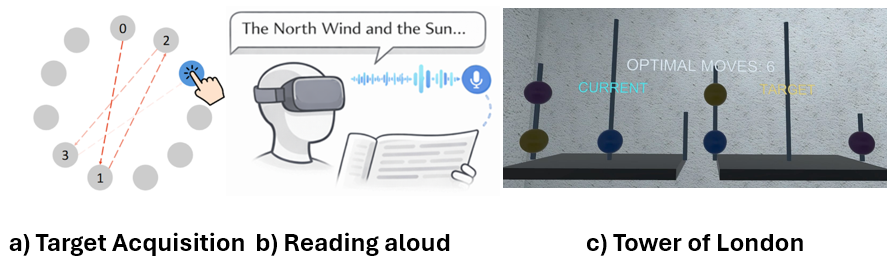
\includegraphics[width=1\linewidth]{Figure/try.png}
    \caption{The tasks used in the experiment: (a) target acquisition; (b) reading aloud; and (c) Tower of London (in-situ VR screenshot).}
    \label{fig:tasks}
\end{figure}
To investigate how acute stress affects different forms of interaction in VR, we implemented three tasks: \textit{target acquisition}, \textit{reading aloud}, and \textit{Tower of London} in a unified immersive environment (~\autoref{fig:tasks}). All tasks were developed in Unity 2022.3.62f3 and deployed on a Meta Quest Pro headset using optical hand tracking (XR Hands) for controller-free interaction. We recorded physiological data with a Polar H10 chest strap.

\subsection{Tasks}
As outlined in Section~\ref{sec:relatedwork}, we used MRT~\cite{wickens2008multiple} as a task-selection framework, rather than as a direct test of resource competition. The three tasks were chosen to sample different combinations of perceptual modality, processing code, response form, and central/executive demand:

\begin{itemize}
    \item \textbf{Target acquisition}: a visual-spatial task with manual response, emphasizing visuomotor coordination and fine motor control with low central planning demands.
    \item \textbf{Reading aloud}: a visual-verbal task with vocal response, emphasizing verbal encoding and speech production under controlled linguistic content.
    \item \textbf{Tower of London}: a visual-spatial task with manual response and substantial central/executive demands, emphasizing sequential planning.
\end{itemize}

Participants performed all tasks while standing, using hand tracking for direct manipulation of virtual objects. Before the experiment, they completed training trials for each task until comfortable with the interaction techniques. Task order was counterbalanced across participants using a Latin square design.

\subsubsection{Target Acquisition Task}
We implemented a target acquisition task using direct hand selection, following the methodology described in ISO 9241-411 for evaluating pointing devices. Eleven spherical targets were arranged in a circular layout 49~cm in front of the participant~\cite{li2025weight}. We instructed participants to select the highlighted targets in a displayed sequence as quickly and as accurately as possible by directly touching each sphere with their index finger. Each round comprised 11 successful selections, with a selection registered when the fingertip entered the 3~cm radius of the target.

To minimise ambiguity, the first target in each sequence was explicitly highlighted and the upcoming target was indicated in advance using a lighter shade. Upon successful selection, the system updated the highlighting to reflect the next target. A cross marker was placed at the centre of each target to indicate the intended selection point and reduce spatial uncertainty. For perceptual clarity and accessibility, all targets were rendered in blue tones, with active and upcoming targets differentiated through luminance rather than hue, avoiding reliance on red-green contrasts.

\subsubsection{Target Acquisition Measures}
We recorded standard pointing performance metrics: movement time, throughput, and endpoint offset, following established evaluation methods~\cite{liu2025understanding}. Movement time (MT) was defined as the elapsed time between consecutive successful selections. Throughput (TP) was computed as a standard Fitts' law efficiency measure:
\[
TP = \frac{ID_e}{MT},
\]
where $ID_e$ is the effective index of difficulty. Endpoint offset was computed as the Euclidean distance between the fingertip and the target centre at the moment of selection:
\[
Offset = \sqrt{(x_f-x_c)^2 + (y_f-y_c)^2 + (z_f-z_c)^2}.
\]
Together, these metrics capture acquisition speed, the speed-accuracy trade-off, and endpoint precision.

We additionally conducted an exploratory trajectory-based analysis of terminal pointing stability. For each successful trial, we computed the fingertip-to-target offset over the final five samples preceding selection and quantified pre-hit stability as their standard deviation:
\[
PreHitStability = \mathrm{SD}(offset_{t-4}, \dots, offset_t).
\]
Lower values indicate more stable endpoint behaviour immediately before acquisition. This measure captures fine-grained terminal variability that may not surface in aggregate outcomes. Prior motor-control work shows that mental calculation can increase postural hand tremor while leaving goal-directed kinetic tremor comparatively unchanged~\cite{budini2022mental}; we therefore treated pre-hit stability as an exploratory indicator of terminal endpoint control rather than as a direct measure of tremor.

\subsubsection{Reading Aloud Task}
We chose reading aloud rather than spontaneous speech as a task to maintain comparable linguistic content across participants and phases while still capturing stress-related changes in vocal production. Participants read excerpts from three phonetically balanced passages widely used in speech research: \textit{The North Wind and the Sun}~\cite{international1999handbook}, \textit{The Rainbow Passage}~\cite{van1972speech}, and the \textit{Grandfather Passage}~\cite{fairbanks1940voice}. To reduce passage-specific repetition and ordering effects, one passage was assigned to each experimental round using random selection without replacement, so that each participant read all three passages exactly once across the three rounds.

For experimental consistency, the passages were trimmed to approximately 110 words while preserving complete sentences, and were selected to have similar Flesch-Kincaid~\cite{kincaid1975derivation} grade levels (6.94, 7.22, and 8.16), indicating broadly comparable reading difficulty. This ensured comparable reading duration across trials while maintaining natural linguistic structure. Passages were displayed as floating text panels in the VR environment, and participants were instructed to read clearly and naturally. Audio and task timestamps were recorded for subsequent analysis.

\subsubsection{Reading Aloud Measures}
We report reading duration, mean fundamental frequency (F0), speech rate, and active speech ratio. To reduce onset hesitation and recording-start artefacts, the first 3~seconds of each recording were excluded from acoustic analysis. Reading duration served as a coarse temporal measure of task completion, while mean F0, speech rate, and active speech ratio were extracted as acoustic indicators of vocal arousal and temporal speech behaviour, following prior work in which speech-based stress and affect analysis commonly relies on prosodic and temporal features~\cite{schewski2025measuring,kappen2022acoustic}.

\subsubsection{Tower of London Task}
We implemented a VR version of the Tower of London (ToL) task~\cite{shallice1982specific} to assess executive planning and sequential problem solving. Participants were presented with an initial arrangement of coloured balls across three pegs together with a target configuration shown nearby, and were instructed to reproduce the target configuration by moving balls between pegs, subject to the constraints that only one ball could be moved at a time and that pegs had limited capacity. Participants manipulated the balls using a pinch gesture~\cite{mikkelsen2025dof}, enabling embodied interaction without controllers. The Unity application logged object states, hand-tracking events from XR Hands, move sequences, and timestamps throughout the task. Each board contained three coloured balls (8~cm in diameter) and three pegs with capacities of three, two, and one ball; adjacent peg centres were separated by 25~cm, and the current and target boards were positioned approximately 60~cm apart. 

To ensure consistent difficulty across rounds,the coloured balls and the pegs shows in random sequence and we used ToL problems with a uniform solution depth of six moves with one rollback structure across rounds, as problem difficulty in the Tower of London is known to depend on both minimum solution length and structural characteristics of the problem~\cite{kaller2004impact}. This design avoided ceiling effects from overly simple problems and floor effects or disproportionate variability from excessively difficult ones~\cite{kaller2012assessing}. 

To minimise direct learning of specific configurations, we varied the spatial arrangement of balls and pegs across rounds while preserving structural difficulty, so participants encountered different instantiations rather than repeating identical layouts. This decision was also informed by pilot testing: with more repeated ToL rounds, repeated exposure substantially reduced errors over time, suggesting that learning effects could overshadow stress-related differences.

\subsubsection{Tower of London Measures}
We report first-move latency, move count, total duration, and execution time. First-move latency was defined as the interval from trial onset to the initiation of the first move, capturing the period during which participants inspected the initial and target configurations and formulated an initial plan~\cite{shallice1982specific}. Move count was the total number of moves required to reach the target configuration, with deviations from the minimum indicating less efficient planning~\cite{kaller2012assessing}. Total duration captured the time taken to complete the entire task~\cite{kaller2012assessing}, and execution time was computed as the difference between total duration and first-move latency, isolating the post-planning execution phase.

\subsection{Procedure}

\subsubsection{Participants}
We recruited 26 participants from the university community. The final analysis included 24 participants (11 female, 13 male) after excluding two with Polar H10 recordings missing. Participants ranged in age from 20 to 31 years ($M = 24.8$, $SD = 3.0$), all reported normal or corrected-to-normal vision and no known motor impairments, and came from a range of disciplines including computer science, nursing, health, design, digital media, and psychology. The sample size is consistent with commonly adopted local standards in HCI experimental studies~\cite{caine2016local}, and recruitment with nearly equal number of male and female participants to avoid gender bias~\cite{van2009stress}.The study was approved by our institutional ethics committee, and all participants provided informed consent prior to the experiment.
\begin{figure*}[!t]
    \centering
    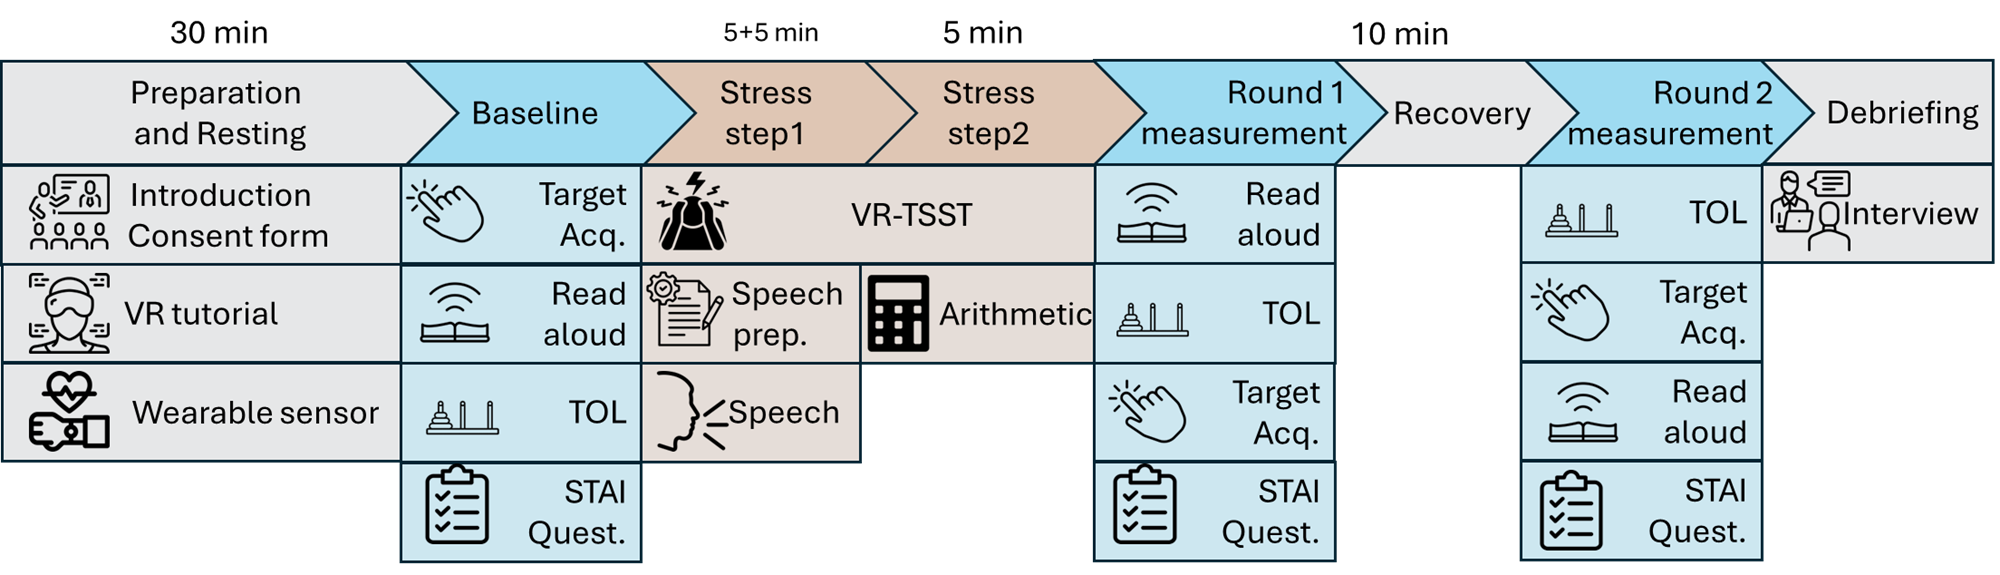
\includegraphics[width=1\textwidth]{Figure/overview.png}
    \caption{Experimental procedure. Abbreviations in the figure: Target Acq. = target acquisition; Speech prep. = speech preparation; Quest. = questionnaire.}
    \label{fig:procedure}
\end{figure*}

To induce stress, we adopted a VR adaptation of the Trier Social Stress Test (VR-TSST). The session comprised four stages: 1) briefing and training, 2) baseline, stress induction with post-stress measurement, and recovery---and lasted approximately 60--70~minutes per participant. An overview is shown in~\autoref{fig:procedure}.

\subsubsection{Preparation and Training}
The experiment took place in the human-centred computing laboratory of our institution. Upon arrival, participants were fitted with a Polar H10 chest strap for physiological data collection. Before fitting the strap, the electrode areas were moistened to improve skin contact, and the strap was positioned around the participant's chest according to the manufacturer's placement guidelines. The sensor was connected via Bluetooth to the recording application, which continuously logged heart-rate estimates and RR intervals throughout the experiment. We first introduced participants to the VR system and they completed a tutorial in which they practised direct finger selection for target acquisition task and pinch gestures for the ToL task. They also rehearsed the ToL rules using a simple example problem and were given a short rest before the formal study began.


\subsubsection{Resting period}
We then left participants alone for 20~minutes to rest and stabilise. During this time we provided them with neutral reading material to keep them occupied without inducing anxiety, as recommended in the TSST protocol~\cite{kirschbaum1993trier}. They subsequently completed the three VR tasks and filled in the STAI-S questionnaire~\cite{spielberger1971state}.

\subsubsection{Stress Induction}
Participants then completed the VR-TSST and were informed that their performance would be video-recorded and reviewed by judges trained in public speaking. They were given 5~minutes to prepare a speech explaining why they would be a suitable candidate for their ideal job, followed by 5~minutes delivering the speech in front of a virtual three-member evaluation committee. Throughout preparation and delivery, the virtual committee members remained present as socially evaluative observers and provided no supportive or encouraging feedback.

Immediately after the speech, participants performed a mental arithmetic task in which they repeatedly subtracted 13 from 1022 and spoke the number sequence aloud~\cite{kirschbaum1993trier}. The same virtual committee remained present throughout, sustaining the socially evaluative atmosphere. Incorrect answers required participants to restart the calculation from the beginning. The subtraction task lasted 5~minutes.

\subsubsection{Post-Stress Measurement (Round 1)}
Immediately after stress induction, participants completed the first post-stress measurement round, again performing the three VR tasks and filling in the STAI questionnaire. Task order differed from the baseline stage to reduce learning effects.

\subsubsection{Recovery and Post-Recovery Measurement (Round 2)}
Following the stress elicitation round, participants were given a 10~minute recovery period. To improve comfort and reduce headset fatigue, they need to remove the headset and rest quietly. After recovery, participants completed the second measurement round and filled in the STAI questionnaire.

\subsubsection{Participant Debriefing}
Finally, we debriefed participants about the study, explained that experiencing stress during the experiment was expected, and clarified that the tasks were intentionally demanding and did not reflect participants' aptitude or ability. We also informed them that their performance had not been evaluated by a real judging panel. We then conducted a short semi-structured interview, asking participants to report their subjective perception of the experiment and the effect of stress on their performance.
\subsection{Stress Validation Measures}
We validated stress occurrence using participants' self-reported anxiety and physiological responses. We measured self-reported anxiety with the state scale of the State-Trait Anxiety Inventory – State scale (STAI-S) after each round~\cite{spielberger1971state}. We recorded physiological responses  with a Polar H10 chest strap. To calculate high-frequency heart rate variability (HF HRV), a frequency-domain measure of heart rate variability (HRV),we extracted heart rate and inter-beat interval (IBI) estimates derived from the RR intervals. Following prior work~\cite{sarsenbayeva2019measuring}, We ordered IBI samples by timestamp, interpolated them to a uniformly sampled 4~Hz time series, and analysed using an Fast Fourier Transform (FFT)-based sliding-window procedure. For each 512-sample window, we computed the frequency spectrum and summed spectral magnitude within the high-frequency band (HF HRV: 0.15--0.40~Hz). HF HRV values were averaged within each physiological analysis window and log-transformed before statistical analysis. In addition to HF HRV, we computed mean heart rate (HR) and the standard deviation of normal-to-normal intervals (SDNN) as indicators of cardiovascular arousal. Although the root mean square of successive differences between normal heartbeats (RMSSD) is often used as an index of parasympathetic activity, the VR-TSST in our study involved continuous speech and aloud arithmetic tasks, which may directly affect short-term beat-to-beat variability. We therefore use SDNN as the primary time-domain HRV measure and treat RMSSD as a complementary measure~\cite{shaffer2017overview}. All physiological data processing and statistical analyses were conducted in Python using custom scripts with pandas, NumPy, SciPy, and Matplotlib.



